\section{Modelo}

\subsection{Modelo inicial de coloreo}
\begin{frame} 
\frametitle{Modelo de coloreo}

Definimos las siguientes variables binarias:

\begin{itemize}
\item{$x_{ij}$ es verdadera sii el v�rtice $i$ es coloreado con el color $j$}
\item{$w_{j}$ es verdadera sii el color $j$ fue usado}
\end{itemize}

\uncover<2>{
\lpobjective{Buscamos minimizar la cantidad de colores distintos usados}
{\min \sum_{j \in C} w_{j}}
}

\end{frame} 

\begin{frame} 
\frametitle{Modelo de coloreo}

Agregamos las restricciones de coloreo:

\begin{itemize}
\item<2->{
\lprestriction{La variable $w_j$ es verdadera sii alg�n v�rtice usa el color $j$}
{x_{ij} \leq w_j}{\forall j \in C, \forall i \in V}
}

\item<3->{
\lprestriction{Dos vecinos no pueden usar el mismo color}
{x_{ij} + x_{kj} \leq 1}{\forall j \in C, \forall (i,k) \in E}
}

\item<4->{
\lprestriction{Cada \only<4>{v�rtice}\alert<5>{\only<5>{partici�n}} tiene exactamente un color asignado}
{\uncover<5>{\sum _{x_i \in p}} \sum_{j \in C} x_{ij} = 1}{\forall i \in V \uncover<5>{, p \in P}}
}
\end{itemize}

\end{frame} 

\begin{frame}
\frametitle{Modelo de coloreo}

Con esto ya tenemos una formulaci�n b�sica del problema que podemos resolver con un algoritmo de branch and cut. Pero podemos reforzar la formulaci�n para mejorar los tiempos de resoluci�n del algoritmo:

\begin{itemize}
\item{expresando las restricciones de adyacencia de otras maneras}
\item{agregando restricciones de eliminacion de simetr�a}
\item{agregando otras desigualdades v�lidas}
\end{itemize}

\end{frame} 

\subsection{Reforzando el modelo}

\begin{frame}
\frametitle{Restricciones de adyacencia}

\begin{itemize}
\item{
\lprestriction{Dado un nodo $i_0$, por cada partici�n vecina, o bien $i_0$ usa el color $j$, o a lo sumo uno de sus vecinos por partici�n puede usarlo.}
{\sum_{i \in P_k \cap N(i_0)} x_{ij} + x_{i_0j} \leq w_j}{\forall j \in C, \; \forall P_k \in P, \; \forall i_0 \in V }
\begin{figure}[h]
\centering
\uncover<2->{\alt<2>{\adjsrestrictionpartone}{\adjsrestrictionparttwo}}
\end{figure}
}
\end{itemize}

\uncover<4>{
\begin{centerblock}{}
Estas restricciones arrojaron los mejores resultados para grafos de alta densidad.
\end{centerblock}
}

\end{frame} 

\begin{frame}
\frametitle{Restricciones de adyacencia}

\begin{itemize}
\item{
\lprestriction{Generalizamos las anteriores pidiendo o bien un nodo $i_0$ usa el color $j$, o bien a lo sumo \alert<3->{$r$} de sus vecinos lo utilizan.}
{\sum_{i \in N(i_0)} x_{i_0j} + \alert<3->{r} * x_{i_0j} \leq \alert<3->{r} * w_j}{\forall j \in C, \; \forall i_0 \in V}
\begin{figure}[h]
\centering
\uncover<2->{\adjsrestrictionneighbours}
\end{figure}
}
\end{itemize}

\uncover<4>{
\begin{centerblock}{}
Estas restricciones arrojaron los mejores resultados para grafos de baja densidad.
\end{centerblock}
}

\end{frame} 

\subsection{Eliminaci�n de simetr�a}
\begin{frame}
\frametitle{Eliminaci�n de simetr�a}

Un problema que tiene este problema, que se traduce al modelo, es que admite muchas soluciones sim�tricas para un mismo grafo:

\begin{figure}[h]
	\centering
	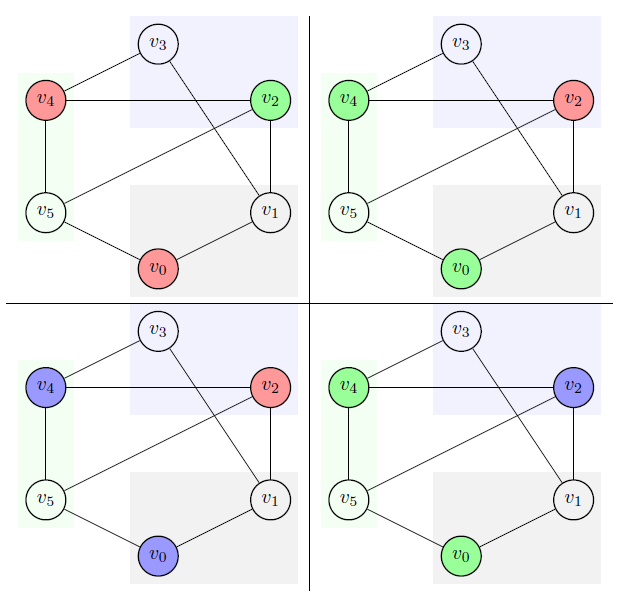
\includegraphics[scale=0.4]{symmetry.png}
\end{figure}

\end{frame} 

\begin{frame}{Eliminaci�n de simetr�a}

Buscamos agregar restricciones al modelo que eliminen soluciones sim�tricas:

\begin{itemize}
\item<2->{
\lprestriction{No se permite usar un color hasta que no se hayan usado todos los anteriores}
{w_j \geq w_{j+1}}{\forall 1 \leq j < c }
}
\end{itemize}

\uncover<3>{Esta restricci�n asegura que s�lo se usen los primeros colores, pero permite soluciones simetr�cas que usan el mismo conjunto de colores.}

\end{frame}

\begin{frame}{Eliminaci�n de simetr�a}

\begin{itemize}
\item{
\lprestriction{La cantidad de nodos coloreados con un color $j_0+1$ no puede ser mayor que la cantidad coloreada con $j_0$.}
{\sum_{i \in V} x_{ij} \geq \sum_{i \in V} x_{ij+1}}{\forall 1 \leq j < c }
}
\end{itemize}

\uncover<2>{Elimina muchas soluciones sim�tricas, pero a�n permite intercambiar colores entre aquellos usados por la misma cantidad de nodos.}

\end{frame}

\begin{frame}{Eliminaci�n de simetr�a}

\begin{itemize}
\item{
\lprestriction{Asignamos el color de menor �ndice al conjunto de nodos que tenga la partici�n de menor �ndice}
{x_{ij} \leq \sum_{l = j-1}^{k-1} \sum_{u \in P_l} x_{uj-1}}{\forall 1 < k \leq q, \; \forall i \in P_k, \; \forall 1 < j \leq k}
}
\item<2->{
\lprestriction{Ninguna partici�n puede estar coloreada con un color de etiqueta mayor a su �ndice}
{x_{ij} = 0}{\forall j > p(i) + 1}
}
\end{itemize}

\uncover<3>{
\begin{centerblock}{}
Este par de restricciones es el que mejores resultados arroj� en el algoritmo implementado.
\end{centerblock}
}

\end{frame}


\begin{frame}
\frametitle{Desigualdades v�lidas en el modelo}

\begin{itemize}

\item{
\lprestriction{Ning�n v�rtice puede usar un color de etiqueta mayor a la cantidad de colores usados.}
{\sum_{j \in C} j x_{ij} \leq \sum_{j \in C} w_j}
{\forall i \in V}
}


\item<2>{
\lprestriction{{\alert{Ninguna partici�n}} puede usar un color de etiqueta mayor a la cantidad de colores usados.}
{\sum_{j \in C} \sum_{i \in P_k} j x_{ij} \leq \sum_{j \in C} w_j}
{\forall P_k \in P}
}

\end{itemize}

\end{frame} 

